\documentclass[a4paper,12pt]{article}
\usepackage[utf8]{inputenc}
\usepackage{polski}
\usepackage{graphicx}
\usepackage{listings}
\author{Marcin Fabrykowski}
\title{Modelowanie procesów fizycznych\\Lab 04-05}
\begin{document}
	\maketitle
	\newpage
	\section{Metoda jawna}
	Została wykorzystana metoda QUICKEST. Charakteryzuje się ona szybkością obliczeń.\\
	Na rysunkach \ref{l4-1}, \ref{l4-2}, \ref{l4-3} przedstawiono rozpływ cieczy fazie początkowej, środkowej oraz końcowej.\\
	Na rysunku \ref{l4-hist} przedstawiono stężenie cieczy w punkcie pomiarowym umieszczonym na pozycji 80
	\begin{figure}
	\hspace{-100px}
	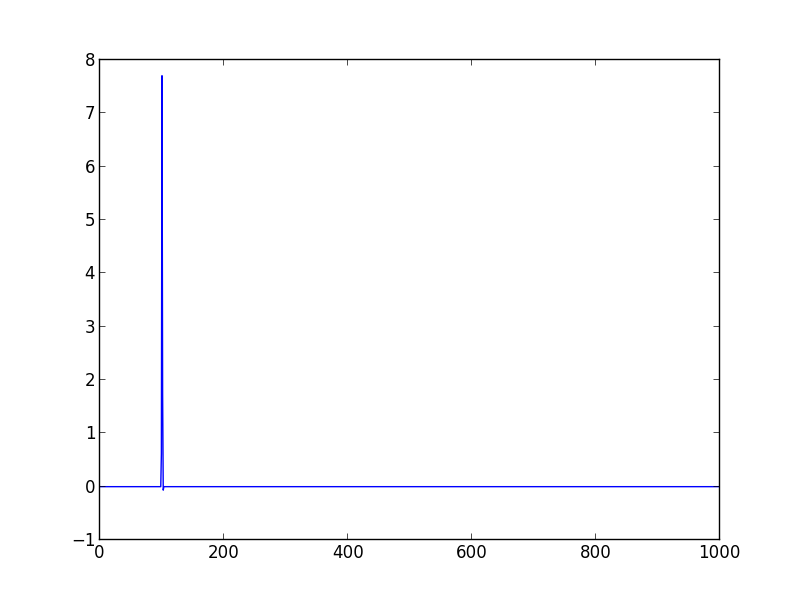
\includegraphics{plots1/00000}
	\caption{Metoda jawna - faza początkowwa}
	\label{l4-1}
	\end{figure}
	\begin{figure}
	\hspace{-100px}
	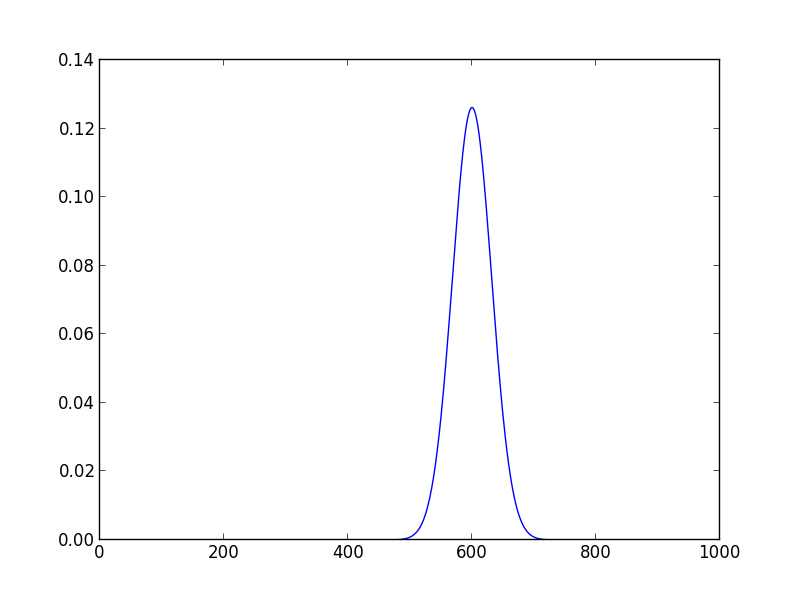
\includegraphics{plots1/00100}
	\caption{Metoda jawna - faza środkowa}
	\label{l4-2}
	\end{figure}
	\begin{figure}
	\hspace{-100px}
	
\includegraphics{plots1/00199}
	\caption{Metoda jawna - faza końcowa}
	\label{l4-3}
	\end{figure}
	\begin{figure}
	\hspace{-100px}
	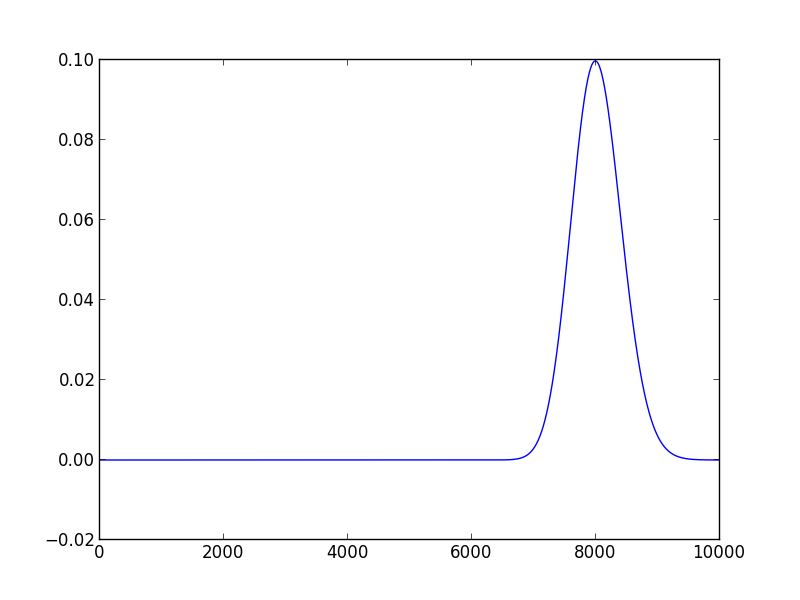
\includegraphics{plots1/hist}
	\caption{Metoda jawna - punk pomiarowy}
	\label{l4-hist}
	\end{figure}
	\section{Metoda niejawna}
	Została wykorzystana metoda Cranka-Nicolsona. Charakteryzuje się ona dokładnością obliczeń.
	Na rysunkach \ref{l5-1}, \ref{l5-2}, \ref{l5-3} przedstawiono rozpływ cieczy fazie początkowej, środkowej oraz końcowej.\\
	Na rysunku \ref{l5-hist} przedstawiono stężenie cieczy w punkcie pomiarowym umieszczonym na pozycji 80
	\begin{figure}
	\hspace{-100px}
	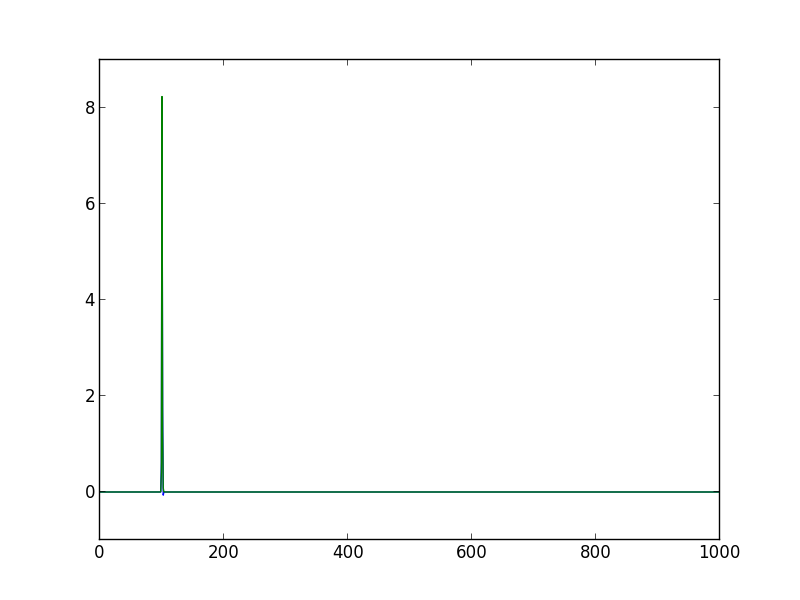
\includegraphics{plots2/00000}
	\caption{Metoda jawna - faza początkowwa}
	\label{l5-1}
	\end{figure}
	\begin{figure}
	\hspace{-100px}
	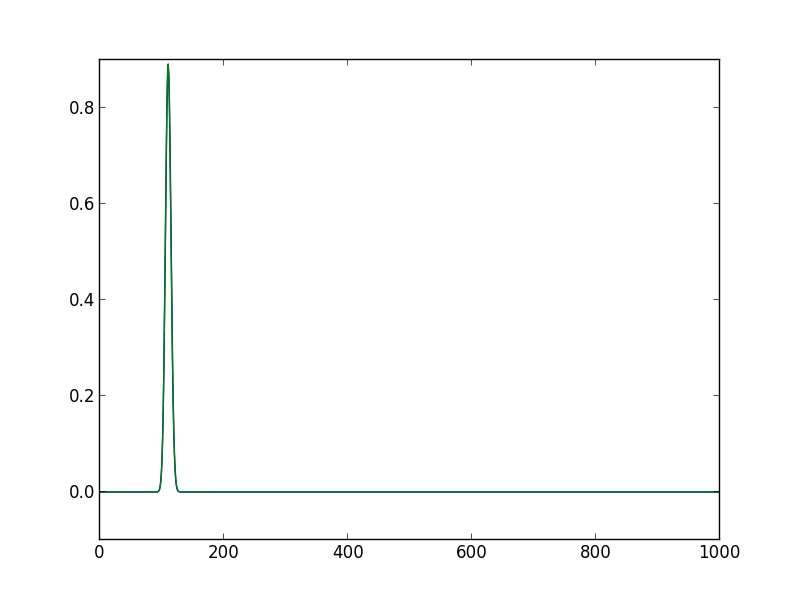
\includegraphics{plots2/00100}
	\caption{Metoda jawna - faza środkowa}
	\label{l5-2}
	\end{figure}
	\begin{figure}
	\hspace{-100px}
	
\includegraphics{plots2/00199}
	\caption{Metoda jawna - faza końcowa}
	\label{l5-3}
	\end{figure}
	\begin{figure}
	\hspace{-100px}
	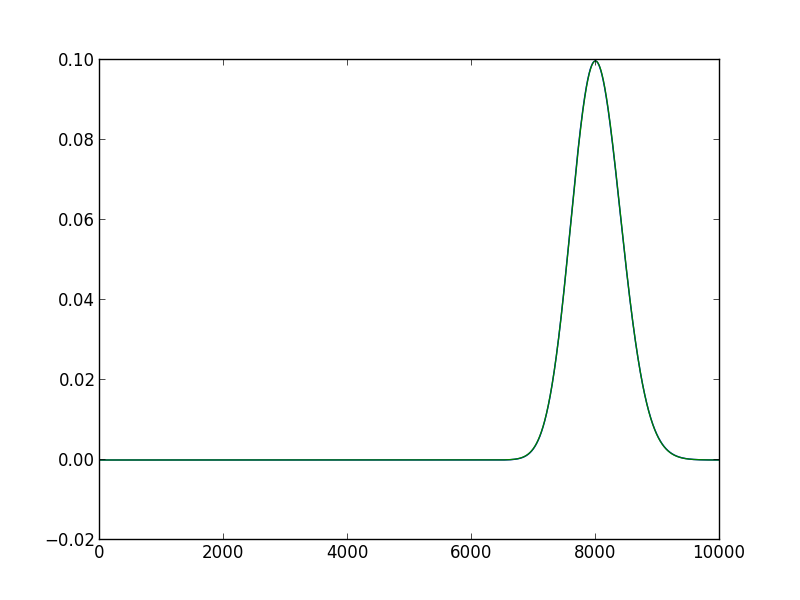
\includegraphics{plots2/hist}
	\caption{Metoda jawna - punk pomiarowy}
	\label{l5-hist}
	\end{figure}
	\section{Kod programu}
	\lstinputlisting[language=python]{lab04.py}
	\section{Wnioski}
	Zauważamy, że obie metody dały bardzo porównywalne wyniki.\\
	Oba algorytmy spełniają zasadę zachowania masy.
\end{document}
